\documentclass[11pt,aspectratio=169]{beamer}

\usepackage{amsmath,amssymb,bm}
\usepackage{booktabs}
\usepackage{tikz}
\usetikzlibrary{arrows.meta,positioning,calc}

\usetheme{default}
\setbeamertemplate{navigation symbols}{}
\setbeamertemplate{headline}{}
\setbeamertemplate{footline}{%
  \leavevmode
  \hbox{%
    \begin{beamercolorbox}[wd=\paperwidth,ht=2.6ex,dp=1.1ex,right]{page number in head/foot}%
      \insertframenumber/\inserttotalframenumber\hspace{0.35cm}
    \end{beamercolorbox}%
  }%
}
\setbeamertemplate{frametitle}{\vspace{0.25cm}\insertframetitle\par\vspace{0.08cm}\hrule}
\setbeamercolor{normal text}{fg=black,bg=white}
\setbeamercolor{frametitle}{fg=black,bg=white}
\setbeamercolor{structure}{fg=black}
\setbeamersize{text margin left=0.7cm,text margin right=0.7cm}

\newcommand{\dd}{\,\mathrm{d}}
\newcommand{\Om}{\Omega}
\newcommand{\GamD}{\Gamma_D}
\newcommand{\GamN}{\Gamma_N}
\newcommand{\Th}{\mathcal T_h}
\newcommand{\Fh}{\mathcal F_h}
\newcommand{\Vzero}{\mathcal V_0}
\newcommand{\Vhzero}{\mathcal V_{h,0}}
\newcommand{\Qh}{\mathcal Q_h}
\newcommand{\Ih}{\mathcal I_h}
\newcommand{\norm}[2][]{\left\lVert#2\right\rVert_{#1}}
\newcommand{\seminorm}[2][]{\left\lvert#2\right\rvert_{#1}}
\newcommand{\grad}{\nabla}
\newcommand{\divg}{\nabla\!\cdot}
\newcommand{\bn}{\bm n}
\newcommand{\bq}{\bm q}
\newcommand{\bx}{\bm x}

\begin{document}

\begin{frame}[plain]
  \centering\vfill
  {\LARGE\bfseries Residual Estimator and Reliability\par}
  \vspace{0.45cm}
  {\large Part 2: independent study\par}
  \vspace{0.25cm}
  {\large Local approximation estimates and an energy-error bound\par}
  \vfill
\end{frame}

\begin{frame}{Reading outline}
Continue after the quasi-interpolation construction in Part 1.
\begin{enumerate}
  \item Identify the element and facet patches and use the two local estimates.
  \item Derive the mesh-size weights, define $\eta_e$ and $\eta$, and
  calculate a two-triangle example.
  \item Combine Cauchy--Schwarz and finite patch overlap to prove reliability.
  \item Return to the nonuniform 1D example and compare indicators with errors.
\end{enumerate}
The local estimates for $\Qh$ are stated as a hypothesis, not proved here.
The remaining slides show how that hypothesis yields the error bound.
\end{frame}

\begin{frame}{Starting identities from Part 1}
Use the same diffusion form and homogeneous Dirichlet test spaces as in Part 1:
\[
 a(w,v)=\int_\Om k\grad w\cdot\grad v\,\dd x,
 \quad \norm[a]{v}=\sqrt{a(v,v)},
 \quad \Vhzero\subset\Vzero.
\]
Here $\ell(v)=\int_\Om fv\,\dd x+\int_{\GamN}qv\,\dd s$ and
$R(u_h;v)=\ell(v)-a(u_h,v)$. With $e=u-u_h$,
\[
 R(u_h;v)=a(e,v),\qquad R(u_h;v_h)=0\quad(v_h\in\Vhzero).
\]
The averaging operator maps $\Qh:\Vzero\to\Vhzero$. Taking $v=e$ and
$v_h=\Qh e$ gives the identity used below:
\[
 \boxed{\norm[a]{e}^2=R(u_h;e-\Qh e).}
\]
\end{frame}

\begin{frame}{The patches in the local estimates}
An \textbf{element patch} $\omega_e$ contains all elements sharing a vertex
with $\mathcal K_e$. A \textbf{facet patch} $\omega_{\mathcal F}$ contains
all elements sharing a vertex with $\mathcal F$.

\begin{columns}[T,onlytextwidth]
\begin{column}{0.48\textwidth}
\centering
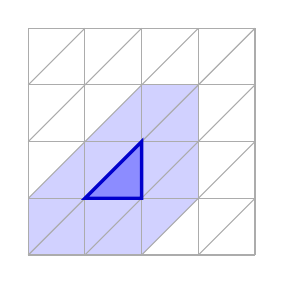
\begin{tikzpicture}[x=0.72cm,y=0.72cm]
 \foreach \a/\b in {1/1,2/1,2/2}{
  \fill[blue!18,shift={(\a,\b)}]
   (-1,-1)--(0,-1)--(1,0)--(1,1)--(0,1)--(-1,0)--cycle;
 }
 \draw[gray!65,step=1] (0,0) grid (4,4);
 \foreach \i in {0,...,3}{\foreach \j in {0,...,3}{
   \draw[gray!65] (\i,\j)--(\i+1,\j+1);
 }}
 \filldraw[fill=blue!45,draw=blue!80!black,very thick]
  (1,1)--(2,1)--(2,2)--cycle;
\end{tikzpicture}

Dark triangle: $\mathcal K_e$

Blue region: $\omega_e$
\end{column}
\begin{column}{0.48\textwidth}
\centering
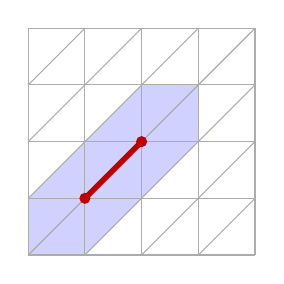
\begin{tikzpicture}[x=0.72cm,y=0.72cm]
 \foreach \a/\b in {1/1,2/2}{
  \fill[blue!18,shift={(\a,\b)}]
   (-1,-1)--(0,-1)--(1,0)--(1,1)--(0,1)--(-1,0)--cycle;
 }
 \draw[gray!65,step=1] (0,0) grid (4,4);
 \foreach \i in {0,...,3}{\foreach \j in {0,...,3}{
   \draw[gray!65] (\i,\j)--(\i+1,\j+1);
 }}
 \draw[red!75!black,line width=2pt] (1,1)--(2,2);
 \fill[red!75!black] (1,1) circle (2pt);
 \fill[red!75!black] (2,2) circle (2pt);
\end{tikzpicture}

Red edge: $\mathcal F$

Blue region: $\omega_{\mathcal F}$
\end{column}
\end{columns}
\vspace{0.12cm}
These neighborhoods appear because each coefficient of $\Qh v$ uses a
vertex patch, rather than a value on one element alone.
\end{frame}

\begin{frame}{Assumptions for the residual error bound}
The estimates below use the following setting, as in Chapter 8.
\begin{itemize}
 \item The mesh consists of affine triangles or tetrahedra. It is
 conforming, boundary fitted, and shape regular. The geometric constants
 then stay bounded as the mesh is refined.
 \item The finite element space is the continuous Lagrange space of fixed
 degree $p\geq1$. In particular, it contains the piecewise-linear
 approximation $\Qh v$.
 \item The coefficient satisfies
 $k|_{\mathcal K_e}\in C^1(\overline{\mathcal K_e})$.
 It may jump between elements. The element divergence and facet fluxes
 can therefore be evaluated separately on each element.
 \item The discrete equations are solved exactly, and the forms are
 evaluated exactly. These assumptions give $R(u_h;v_h)=0$ for all
 $v_h\in\Vhzero$.
\end{itemize}
\end{frame}

\begin{frame}{Local approximation estimates for $\Qh$}
For a shape-regular mesh in $d=2$ or $3$, use the following standard
quasi-interpolation estimates for $v\in\Vzero$:
\[
\boxed{\begin{aligned}
 \norm[L^2(\mathcal K_e)]{v-\Qh v}
 &\leq C_Q h_e\seminorm[H^1(\omega_e)]{v},\\[3pt]
 \norm[L^2(\mathcal F)]{v-\Qh v}
 &\leq C_Q h_{\mathcal F}^{1/2}
              \seminorm[H^1(\omega_{\mathcal F})]{v}.
\end{aligned}}
\]
Here $h_e=\operatorname{diam}(\mathcal K_e)$,
$h_{\mathcal F}=\operatorname{diam}(\mathcal F)$, and
\[
 \seminorm[H^1(\omega)]{v}
 =\left(\int_\omega|\grad v|^2\,\dd x\right)^{1/2}.
\]
The constant $C_Q$ does not depend on mesh size. We use these estimates
without proving them. They are Hypothesis (Q) in Chapter 8.

\vspace{0.12cm}
{\footnotesize Sch\"oberl, \S4.3, Theorem 75, p.~65. The element and facet
powers are $h_e$ and $h_{\mathcal F}^{1/2}$, respectively.}
\end{frame}

\begin{frame}{Applying the subtraction identity to the error}
The operator gives $\Qh e\in\Vhzero$. Set $v_h=\Qh e$ in
the subtraction identity:
\[
\begin{aligned}
 \norm[a]{e}^2
 &=R(u_h;e)\\
 &=R(u_h;e)-\underbrace{R(u_h;\Qh e)}_{0}\\
 &=R(u_h;e-\Qh e).
\end{aligned}
\]
Write $w=e-\Qh e\in\Vzero$. Substituting this particular test function into the
element-and-facet residual representation gives
\[
 \boxed{\norm[a]{e}^2
 =\sum_{e'}\int_{\mathcal K_{e'}}r_{e'}w\,\dd x
 +\sum_{\mathcal F\in\Fh^{\mathrm{int}}\cup\Fh^N}
            \int_{\mathcal F}j_{\mathcal F}w\,\dd s.}
\]
Neither $e$ nor $\Qh e$ is computed when evaluating the estimator.
\end{frame}

\begin{frame}{The element term produces the weight $h_e$}
Recall $w=e-\Qh e$. For one element $\mathcal K_{e'}$,
\[
\begin{aligned}
\left|\int_{\mathcal K_{e'}}r_{e'} w\,\dd x\right|
&\leq
\norm[L^2(\mathcal K_{e'})]{r_{e'}}
\norm[L^2(\mathcal K_{e'})]{w}\\[4pt]
&\leq
C_Q\,
\underbrace{h_{e'}\norm[L^2(\mathcal K_{e'})]{r_{e'}}}_{
\text{computable weighted element residual}}
\seminorm[H^1(\omega_{e'})]{e}.
\end{aligned}
\]
Use Cauchy--Schwarz on $\mathcal K_{e'}$, then the element estimate with
$v=e$, for which $v-\Qh v=w$.

The square of the computable factor is
\[
  \left(h_{e'}\norm[L^2(\mathcal K_{e'})]{r_{e'}}\right)^2
  =h_{e'}^2\norm[L^2(\mathcal K_{e'})]{r_{e'}}^2.
\]
This is the element contribution used in the estimator.
\end{frame}

\begin{frame}{The facet term produces the weight $h_{\mathcal F}^{1/2}$}
For one interior or Neumann facet,
\[
\begin{aligned}
\left|\int_{\mathcal F}j_{\mathcal F}w\,\dd s\right|
&\leq
\norm[L^2(\mathcal F)]{j_{\mathcal F}}
\norm[L^2(\mathcal F)]{w}\\
&\leq C_Q\,
\underbrace{h_{\mathcal F}^{1/2}
\norm[L^2(\mathcal F)]{j_{\mathcal F}}}_{
\text{computable weighted facet residual}}
\seminorm[H^1(\omega_{\mathcal F})]{e}.
\end{aligned}
\]
Use Cauchy--Schwarz on $\mathcal F$, then the facet estimate with $v=e$,
for which $v-\Qh v=w$.

The square of the computable factor is
\[
  \left(h_{\mathcal F}^{1/2}\norm[L^2(\mathcal F)]{j_{\mathcal F}}\right)^2
  =h_{\mathcal F}\norm[L^2(\mathcal F)]{j_{\mathcal F}}^2.
\]
This is the facet contribution used in the estimator.
\end{frame}

\begin{frame}{The global residual estimator}
Let
\[
  \Fh^\ast=\Fh^{\mathrm{int}}\cup\Fh^N.
\]
For $d=2$ or $3$, define the \textbf{global residual estimator} by collecting
the squared computable factors from the two bounds:
\[
\boxed{
  \eta^2=
  \sum_e h_e^2\norm[L^2(\mathcal K_e)]{r_e}^2
  +\sum_{\mathcal F\in\Fh^\ast}
   h_{\mathcal F}\norm[L^2(\mathcal F)]{j_{\mathcal F}}^2.}
\]
Every quantity in $\eta$ is computable from the mesh, the data, and $u_h$.

The reliability proof will compare $\eta$ with the unknown energy error.
\end{frame}

\begin{frame}{Local indicators distribute the global estimator}
For each element $\mathcal K_e$, define the \textbf{local error indicator} by
\[
\boxed{
\begin{aligned}
\eta_e^2={}&h_e^2\norm[L^2(\mathcal K_e)]{r_e}^2
+\frac12\sum_{\substack{\mathcal F\subset\partial\mathcal K_e\\
\mathcal F\in\Fh^{\mathrm{int}}}}
h_{\mathcal F}\norm[L^2(\mathcal F)]{j_{\mathcal F}}^2\\
&+\sum_{\substack{\mathcal F\subset\partial\mathcal K_e\\
\mathcal F\in\Fh^N}}
h_{\mathcal F}\norm[L^2(\mathcal F)]{j_{\mathcal F}}^2.
\end{aligned}
}
\]
On summing over elements, each interior contribution has total weight
$1/2+1/2=1$. Each Neumann contribution is counted once. Hence
\[
  \eta^2=\sum_e\eta_e^2.
\]
The values $\eta_e$ help select elements for refinement. They are not exact
local errors.
\end{frame}

\begin{frame}{Two-triangle example: zero element residuals}
\small
Consider $-\Delta u=0$ on $\Om=(0,1)^2$, with Dirichlet values shown at
the four vertices and varying linearly along each boundary edge. Use the
two $P_1$ triangles shown below.

\begin{columns}[T,onlytextwidth]
\begin{column}{0.42\textwidth}
\centering
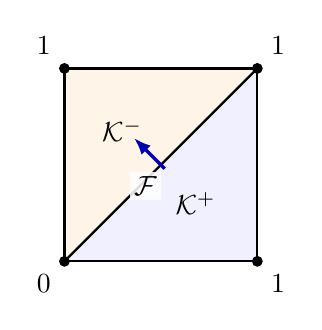
\begin{tikzpicture}[scale=2.45]
  \fill[blue!6] (0,0)--(1,0)--(1,1)--cycle;
  \fill[orange!9] (0,0)--(1,1)--(0,1)--cycle;
  \draw[thick] (0,0) rectangle (1,1);
  \draw[thick] (0,0)--(1,1);
  \foreach \x/\y in {0/0,1/0,1/1,0/1}{\fill (\x,\y) circle (0.8pt);}
  \node[below left=2pt] at (0,0) {$0$};
  \node[below right=2pt] at (1,0) {$1$};
  \node[above right=2pt] at (1,1) {$1$};
  \node[above left=2pt] at (0,1) {$1$};
  \node at (0.68,0.30) {$\mathcal K^+$};
  \node at (0.30,0.68) {$\mathcal K^-$};
  \draw[-{Latex[length=2.2mm]},very thick,blue!70!black]
    (0.52,0.48)--(0.36,0.64);
  \node[fill=white,fill opacity=0.86,text opacity=1,inner sep=1.5pt]
    at (0.42,0.39) {$\mathcal F$};
\end{tikzpicture}

\vspace{0.1cm}
$\displaystyle \bn_{\mathcal F}=\frac{(-1,1)}{\sqrt2}$
\end{column}
\begin{column}{0.55\textwidth}
All vertices lie on the boundary. The unique linear function matching
the three nodal values on each triangle is
\[
  u_h^+(x_1,x_2)=x_1,
  \qquad
  u_h^-(x_1,x_2)=x_2.
\]
Therefore,
\[
  \grad u_h^+=(1,0),
  \qquad
  \grad u_h^-=(0,1).
\]
Because $f=0$ and these gradients are constant,
\[
  r_\pm=\divg(\grad u_h^\pm)=0.
\]
The boundary data are imposed exactly, so $e=0$ on $\partial\Om$.
\end{column}
\end{columns}
\end{frame}

\begin{frame}{Compute the facet term and the local indicators}
Using the normal shown on the previous slide,
\[
\begin{aligned}
  j_{\mathcal F}
  &=-\bigl(\grad u_h^+-\grad u_h^-\bigr)\cdot\bn_{\mathcal F} \\
  &=-\bigl((1,0)-(0,1)\bigr)\cdot
      \frac{(-1,1)}{\sqrt2}
   =\sqrt2.
\end{aligned}
\]
The diagonal has length $h_{\mathcal F}=\sqrt2$, so
\[
  \norm[L^2(\mathcal F)]{j_{\mathcal F}}^2
  =\int_{\mathcal F}2\,\dd s=2\sqrt2,
  \qquad
  \eta^2=h_{\mathcal F}
  \norm[L^2(\mathcal F)]{j_{\mathcal F}}^2=4.
\]
The shared-facet contribution is divided equally between its two neighboring
elements:
\[
  \eta_+^2=\eta_-^2=0+\frac12\,(4)=2,
  \qquad
  \eta^2=\eta_+^2+\eta_-^2.
\]

Since $r_\pm=0$ and there are no Neumann facets, the residual formula reduces
to $R(u_h;v)=\sqrt2\int_{\mathcal F}v\,\dd s$. For example,
$v=x_1(1-x_1)x_2(1-x_2)$ is zero on $\partial\Om$ and positive inside
$\mathcal F$, so $R(u_h;v)>0$. Element terms alone miss this residual.
\end{frame}

\section{Reliability}

\begin{frame}[plain]
  \centering\vfill
  {\LARGE\bfseries Reliability of the estimator\par}
  \vspace{0.4cm}
  {\large Combine the weighted residual bounds and obtain a global
  energy-error estimate\par}
  \vfill
\end{frame}

\begin{frame}{Combining the weighted residual bounds}
With $w=e-\Qh e$ and $\Fh^\ast=\Fh^{\mathrm{int}}\cup\Fh^N$, start from
\[
\begin{aligned}
 \norm[a]{e}^2
 &=\sum_{e'}\int_{\mathcal K_{e'}}r_{e'}w\,\dd x
   +\sum_{\mathcal F\in\Fh^\ast}\int_{\mathcal F}j_{\mathcal F}w\,\dd s\\
 &\leq\sum_{e'}\left|\int_{\mathcal K_{e'}}r_{e'}w\,\dd x\right|
   +\sum_{\mathcal F\in\Fh^\ast}
                  \left|\int_{\mathcal F}j_{\mathcal F}w\,\dd s\right|.
\end{aligned}
\]
Apply the element and facet bounds to these absolute values:
\[
\begin{aligned}
 \norm[a]{e}^2\leq C_Q\Bigg[&
 \sum_{e'} h_{e'}\norm[L^2(\mathcal K_{e'})]{r_{e'}}
          \seminorm[H^1(\omega_{e'})]{e}\\[3pt]
 &+\sum_{\mathcal F\in\Fh^\ast}h_{\mathcal F}^{1/2}
 \norm[L^2(\mathcal F)]{j_{\mathcal F}}
 \seminorm[H^1(\omega_{\mathcal F})]{e}\Bigg].
\end{aligned}
\]
\end{frame}

\begin{frame}{The two lists in Cauchy--Schwarz}
For nonnegative numbers $A_i$ and $B_i$, Cauchy--Schwarz gives
\[
 \sum_i A_iB_i\leq
 \left(\sum_i A_i^2\right)^{1/2}
 \left(\sum_i B_i^2\right)^{1/2}.
\]
Use one combined list, with an entry for every element and every facet:
\begin{center}
\renewcommand{\arraystretch}{1.8}
\begin{tabular}{ccc}
\toprule
Entry & $A_i$: weighted residual & $B_i$: patch seminorm\\
\midrule
Element $e'$ & $h_{e'}\norm[L^2(\mathcal K_{e'})]{r_{e'}}$
 & $\seminorm[H^1(\omega_{e'})]{e}$\\
Facet $\mathcal F$ & $h_{\mathcal F}^{1/2}\norm[L^2(\mathcal F)]{j_{\mathcal F}}$
 & $\seminorm[H^1(\omega_{\mathcal F})]{e}$\\
\bottomrule
\end{tabular}
\end{center}
The sum $\sum_i A_iB_i$ is exactly the bracket in the preceding bound.
\end{frame}

\begin{frame}{Applying Cauchy--Schwarz to both residual sums}
Substitute the entries in the table into
$\norm[a]{e}^2\leq C_Q\sum_i A_iB_i$ and apply Cauchy--Schwarz:
\[
\begin{aligned}
 \norm[a]{e}^2\leq C_Q\,
 &\underbrace{\left(
 \sum_{e'}h_{e'}^2\norm[L^2(\mathcal K_{e'})]{r_{e'}}^2
 +\sum_{\mathcal F\in\Fh^\ast}
 h_{\mathcal F}\norm[L^2(\mathcal F)]{j_{\mathcal F}}^2
 \right)^{1/2}}_{\eta}\\[3pt]
 {}\times{}&\left(\sum_{e'}\seminorm[H^1(\omega_{e'})]{e}^2
 +\sum_{\mathcal F\in\Fh^\ast}
  \seminorm[H^1(\omega_{\mathcal F})]{e}^2\right)^{1/2}.
\end{aligned}
\]
The first factor is exactly the estimator already defined. The remaining
task is to bound the sum of the patch seminorms.
\end{frame}

\begin{frame}{Finite patch overlap gives a global error norm}
Let $m_{e'}$ be the number of element and facet patches containing
$\mathcal K_{e'}$. Shape regularity gives a mesh-independent bound
$m_{e'}\leq N_{\mathrm{ov}}$. Expand each squared seminorm as an integral:
\[
\begin{aligned}
 &\sum_{e'}\seminorm[H^1(\omega_{e'})]{e}^2
  +\sum_{\mathcal F\in\Fh^\ast}
   \seminorm[H^1(\omega_{\mathcal F})]{e}^2\\
 &=\sum_{e'}m_{e'}\int_{\mathcal K_{e'}}|\grad e|^2\,\dd x\\
 &\leq N_{\mathrm{ov}}\sum_{e'}
                 \int_{\mathcal K_{e'}}|\grad e|^2\,\dd x
  =N_{\mathrm{ov}}\seminorm[H^1(\Om)]{e}^2.
\end{aligned}
\]
Thus each element integral is counted at most $N_{\mathrm{ov}}$ times.
Take the square root and substitute into the second Cauchy--Schwarz factor:
\[
  \norm[a]{e}^2
  \leq C_Q\sqrt{N_{\mathrm{ov}}}\,\eta
  \seminorm[H^1(\Om)]{e}.
\]
\end{frame}

\begin{frame}{Reliability of the residual estimator}
Since $k(\bx)\geq k_0>0$, the $H^1$ seminorm satisfies
\[
 \seminorm[H^1(\Om)]{e}^2
 =\int_\Om|\grad e|^2\,\dd x
 \leq\frac1{k_0}\int_\Om k|\grad e|^2\,\dd x
 =\frac1{k_0}\norm[a]{e}^2.
\]
In $\norm[a]{e}^2\leq C_Q\sqrt{N_{\mathrm{ov}}}\,\eta
\seminorm[H^1(\Om)]{e}$, replace the seminorm by
$\norm[a]{e}/\sqrt{k_0}$:
\[
 \norm[a]{e}^2\leq
 C_Q\sqrt{\frac{N_{\mathrm{ov}}}{k_0}}\,\eta\,\norm[a]{e}.
\]
If $e\neq0$, divide by $\norm[a]{e}$. If $e=0$, the bound is immediate:
\[
  \boxed{\norm[a]{u-u_h}\leq
  C_Q\sqrt{\frac{N_{\mathrm{ov}}}{k_0}}\,\eta.}
\]
This is the reliability bound, with
$C_{\mathrm{rel}}=C_Q\sqrt{N_{\mathrm{ov}}/k_0}$ independent of mesh size.
\end{frame}

\begin{frame}{What reliability tells us}
The result just proved is
\[
 \norm[a]{u-u_h}\leq C_{\mathrm{rel}}\eta.
\]
On a shape-regular mesh family, $C_{\mathrm{rel}}$ stays fixed as the mesh
is refined. Consequently,
\[
 \eta\longrightarrow0\quad\Longrightarrow\quad
 \norm[a]{u-u_h}\longrightarrow0.
\]
The computed $\eta$ is \emph{not itself} a guaranteed numerical upper bound:
the theorem contains the constant $C_{\mathrm{rel}}$, which we have not
computed.

Likewise, $\eta_e$ is a contribution to the estimator, not the exact error
on $\mathcal K_e$. Reliability is a global statement. A separate estimate is
needed to compare $\eta_e$ with the error on its surrounding patch.
\end{frame}

\begin{frame}{Recall the nonuniform 1D example}
The problem and computed nodal values from Part 1 are
\[
 -u''=1\text{ on }(0,1),\qquad u(0)=0,\quad u'(1)=0,
\]
\[
 (x_1,x_2,x_3)=(0,1/3,1),\qquad
 (U_1,U_2,U_3)=(0,5/18,1/2).
\]
The element lengths and slopes are
\[
 (h_1,h_2)=(1/3,2/3),\qquad
 (u_h'|_{\mathcal K_1},u_h'|_{\mathcal K_2})=(5/6,1/3).
\]
Thus $r_1=r_2=1$, the interior nodal residual is $j_2=-1/2$, and the
Neumann residual is $j_3=-1/3$. For $v(0)=0$,
\[
 R(u_h;v)=\int_{\mathcal K_1}v\,\dd x+
 \int_{\mathcal K_2}v\,\dd x-\tfrac12v(x_2)-\tfrac13v(x_3).
\]
\end{frame}

\begin{frame}{Returning to 1D: the nodal terms in the error bound}
On an interval, $e\in H^1(0,1)$ has nodal values. We can choose
$v_h=\Ih e\in\Vhzero$ and set $w=e-\Ih e$. At each node,
$w(x_i)=e(x_i)-(\Ih e)(x_i)=0$.

Start from the subtraction identity, then use the 1D residual formula:
\[
\begin{aligned}
 \norm[a]{e}^2
 &=R(u_h;e)-\underbrace{R(u_h;\Ih e)}_{0}=R(u_h;w)\\
 &=\sum_{e'=1}^2\int_{\mathcal K_{e'}}r_{e'}w\,\dd x
   \underbrace{-\frac12w(x_2)-\frac13w(x_3)}_{0}\\
 &\leq\sum_{e'=1}^2\norm[L^2(\mathcal K_{e'})]{r_{e'}}
                         \norm[L^2(\mathcal K_{e'})]{w}.
\end{aligned}
\]
The last step uses Cauchy--Schwarz on each element. The nodal residuals
are nonzero, but their products with $w(x_i)$ vanish.
\end{frame}

\begin{frame}{The 1D interpolation bound and Cauchy--Schwarz}
For linear nodal interpolation on an interval, use the estimate
\[
 \norm[L^2(\mathcal K_{e'})]{v-\Ih v}
 \leq h_{e'}\norm[L^2(\mathcal K_{e'})]{\mathrm dv/\mathrm dx},
 \qquad v\in H^1(0,1).
\]
Use this estimate from Chapter 8 without proof. Set $v=e$, so
$v-\Ih v=w$, then apply Cauchy--Schwarz to the sum:
\[
\begin{aligned}
 \norm[a]{e}^2
 &\leq\sum_{e'=1}^2h_{e'}\norm[L^2(\mathcal K_{e'})]{r_{e'}}
                  \norm[L^2(\mathcal K_{e'})]{\mathrm de/\mathrm dx}\\
 &\leq\underbrace{\left(\sum_{e'=1}^2
 h_{e'}^2\norm[L^2(\mathcal K_{e'})]{r_{e'}}^2\right)^{1/2}}_{
 \eta_{\mathrm{1D}}}
 \left(\sum_{e'=1}^2\norm[L^2(\mathcal K_{e'})]{\mathrm de/\mathrm dx}^2
 \right)^{1/2}.
\end{aligned}
\]
Since the elements partition $(0,1)$ and $k=1$, the last factor is
$\norm[L^2(0,1)]{\mathrm de/\mathrm dx}=\norm[a]{e}$.
Cancel $\norm[a]{e}$ when nonzero to obtain
$\norm[a]{e}\leq\eta_{\mathrm{1D}}$. For $e=0$, this bound is immediate.
\end{frame}

\begin{frame}{The actual element errors in the 1D example}
The exact solution is $u(x)=x-x^2/2$: it satisfies $-u''=1$, $u(0)=0$,
and $u'(1)=0$. Thus $u'=1-x$. Subtract the two computed slopes:
\[
 (u-u_h)'=\begin{cases}
 (1-x)-5/6=1/6-x,&x\in\mathcal K_1=(0,1/3),\\
 (1-x)-1/3=2/3-x,&x\in\mathcal K_2=(1/3,1).
 \end{cases}
\]
Since $k=1$, integrate the square to obtain each local energy error:
\[
\begin{aligned}
 \int_{\mathcal K_1}|u'-u_h'|^2\,\dd x
 &=\int_0^{1/3}(x-1/6)^2\,\dd x
 =\left[\frac{(x-1/6)^3}{3}\right]_0^{1/3}=\frac1{324},\\[4pt]
 \int_{\mathcal K_2}|u'-u_h'|^2\,\dd x
 &=\int_{1/3}^1(x-2/3)^2\,\dd x
 =\left[\frac{(x-2/3)^3}{3}\right]_{1/3}^1=\frac8{324}.
\end{aligned}
\]
\end{frame}

\begin{frame}{Element size in the same 1D example}
Recall $h_1=1/3$, $h_2=2/3$, and $r_1=r_2=1$. For each element, the
squared contribution to $\eta_{\mathrm{1D}}$ is
\[
 h_e^2\norm[L^2(\mathcal K_e)]{r_e}^2
 =h_e^2\int_{\mathcal K_e}1\,\dd x
 =h_e^2h_e=h_e^3.
\]
Compare these contributions with the squared errors just calculated:
\begin{center}
\begin{tabular}{cccc}
\toprule
Element & $h_e$ & $h_e^3$ & $\displaystyle\int_{\mathcal K_e}|u'-u_h'|^2\,\dd x$\\
\midrule
$\mathcal K_1$ & $1/3$ & $1/27$ & $1/324$\\[2pt]
$\mathcal K_2$ & $2/3$ & $8/27$ & $8/324$\\
\bottomrule
\end{tabular}
\end{center}
Here $h_2=2h_1$, so $h_2^3/h_1^3=2^3=8$. The squared local errors
also have ratio $8$. The residuals are equal, but element size makes the
longer element contribute more to both the estimator and the error.
\end{frame}

\begin{frame}{Summary and further reading}
\begin{itemize}
  \item $R(u_h;v)=a(u-u_h,v)$ connects the computable residual functional to
  the unknown error.
  \item Elementwise integration by parts separates balance defects inside
  elements from flux defects on interior and Neumann facets.
  \item Galerkin orthogonality gives $R(u_h;v)=R(u_h;v-\Qh v)$.
  Local approximation estimates then supply the powers of the mesh size.
  \item The indicators $\eta_e$ identify where the residual is concentrated,
  while reliability bounds the global energy error by $C_{\mathrm{rel}}\eta$.
\end{itemize}

\vspace{0.2cm}
\textbf{Exit question.} For $P_1$ elements with elementwise-constant $k$ and
$f=0$, can $\eta$ still be nonzero? Identify the residual term that remains.

\vspace{0.2cm}
\textbf{Part 3 reading.} Interpret reliability, efficiency, and effectivity,
then use the indicators in a solve--estimate--mark--refine loop.
\end{frame}

\begin{frame}{References for the construction and estimates}
\begin{itemize}
 \item J.~Sch\"oberl, \emph{Numerical Methods for Partial Differential
 Equations}, \S4.3, pp.~64--67. Definition 74 gives the patch-average
 construction. Theorems 75--76 give its local estimates and reliability.
 \href{https://jschoeberl.github.io/iFEM/aposteriori/residualEE.html}{Online version: \S27.1--27.2.}
 \item D.~N.~Arnold, \emph{Lecture Notes on Numerical Analysis of Partial
 Differential Equations}, Chapter 4, \S9.1--9.4, pp.~67--73.
 Equations (4.16)--(4.18) give local estimates for a projection-based
 Cl\'{e}ment operator. Equations (4.19)--(4.21) derive the residual bound.
 \item M.~G.~Larson and F.~Bengzon, \emph{The Finite Element Method:
 Theory, Implementation, and Practice}, \S4.9.1, pp.~88--89,
 Theorem 4.7. See also \S2.6.1, pp.~38--39, for the 1D argument.
\end{itemize}
The references develop the homogeneous Dirichlet case. Our proof retains
the Neumann residual and uses the boundary-preserving estimates stated in
Chapter 8 as Hypothesis (Q).
\end{frame}


\end{document}
